\section{Распространённые операторы для битовых строк, отбора.}

Оператор мутации:

\begin{itemize}
      \item Локальная - инвертируем один случайный бит
      \item Глобальная – инвертировать каждый бит с вероятностью 1/(длина строки)
   \end{itemize}

Оператор скрещивание:

\begin{itemize}
      \item Одноточечное
      \item Двуточечное
      \item Однородное
   \end{itemize}

На рисунке снизу для каждого типа скрещивания сверху 2 родителя, а ниже 2 потомка. 

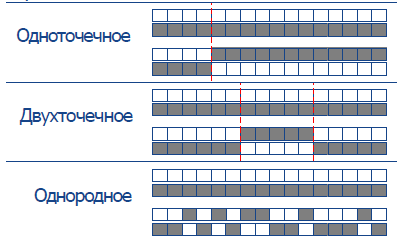
\includegraphics[width=8cm]{images/14bilet.png}  

Оператор отбора для размножения:

\begin{itemize}
      \item Оператор рулетки - каждое решение выбирается с вероятностью, пропорциональной его приспособленности.
      \item Масштабированная рулетка - приспособленность масштабируется линейно.
      \item Турнирный отбор – взять лучшее из N случайных решений.
      \item Позиционно-зависимый отбор – решения сортируются по приспособленности, вероятность выбора зависит от индекса в отсортированной последовательности.
   \end{itemize}

Оператор отбора на выживание:

\begin{itemize}
      \item Схема “плюс” - выбрать лучших из всех особей
      \item Схема “запятая” -  выбрать лучших из потомков
      \item Элитизм -  выбрать p\%  лучших родителей, остальное добрать потомками.
   \end{itemize}